\documentclass{article}
\usepackage[LGR, T1]{fontenc}
\usepackage[greek]{babel}
\usepackage{cancel}
\usepackage{amsmath}
\usepackage{tikz}
\usepackage{alltt}
\usetikzlibrary{trees}
\begin{document}
\title{\textlatin{question2}}
\maketitle
\section*{ΑΠΑΝΤΗΣΗ:}
Παρακάτω έχουμε το αρχικό δέντρο:
\begin{figure}[h]
    \centering
    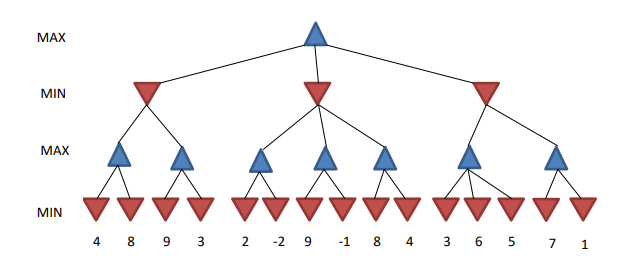
\includegraphics[width=1\linewidth]{image.png}
\end{figure}
\\
Τρέχοντας τον αλγόριθμο \textlatin{minimax}, οι κόμβοι στο επίπεδο 3, ως κόμβοι \textlatin{MAX}, θα λάβουν την μέγιστη τιμή από τα παιδιά τους:
\begin{figure}[h]
    \centering
    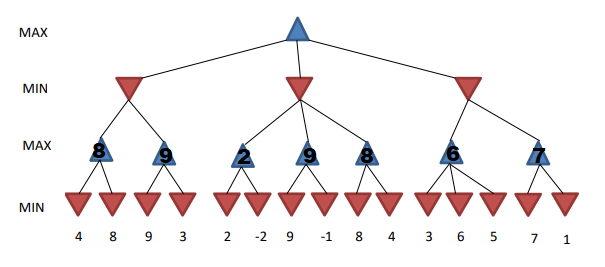
\includegraphics[width=1\linewidth]{image2.png}
\end{figure}
\\
Αντίστοιχα οι \textlatin{MIN} κόμβοι του 2ου επιπέδου θα λάβουν την μέγιστη τιμή από τα παιδιά τους. Τέλος, ο κόμβος-ρίζα που είναι \textlatin{MAX} θα πάρει την μέγιστη τιμή που θα καθορίσει και την \textlatin{minimax} απόφαση στη ρίζα του δέντρου όπως βλέπουμε στην συνέχεια.
\\
\begin{figure}[h]
    \centering
    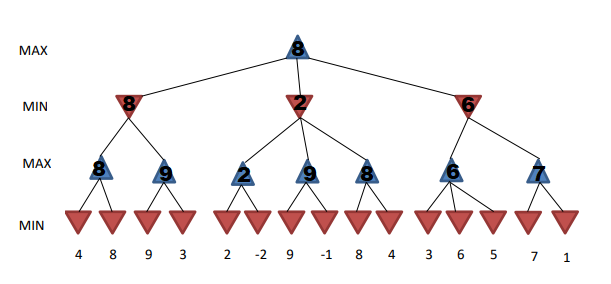
\includegraphics[width=1\linewidth]{image3.png}
\end{figure}
\\
Η \textlatin{minimax} απόφαση στη ρίζα είναι η επιλογή του δεξιότερου κόμβου.
\\\\
Τώρα θα τρέξουμε τον αλγόριθμο \textlatin{ALPHA-BETA-SEARCH} για να δούμε ποιοι κόμβοι θα κλαδευτούν. Στην επόμενη σελίδα παρατίθεται η εκτέλεση του αλγορίθμου θεωρητικά. Η στοίχιση των γραμμών είναι πολύ σημαντική καθώς δηλώνει το βάθος και σε ποιο α-β αναφερόμαστε.
\pagebreak
\begin{alltt}
Επισκεπτόμαστε τον κόμβο \textlatin{A} (\textlatin{MAX}) [α=-\(\infty\), β=\(\infty\)]
  Επισκεπτόμαστε τον κόμβο \textlatin{B} (\textlatin{MIN}) [α=-\(\infty\), β=\(\infty\)]
    Επισκεπτόμαστε τον κόμβο \textlatin{E} (\textlatin{MAX}) [α=-\(\infty\), β=\(\infty\)]
      Επισκεπτόμαστε το φύλλο \textlatin{L} (\textlatin{MIN}) με τιμή 4
    \textlatin{updated alpha}: α=4, β=\(\infty\)
      Επισκεπτόμαστε το φύλλο \textlatin{M} (\textlatin{MIN}) με τιμή 8
    \textlatin{updated alpha}: α=8, β=\(\infty\)
    Ο κόμβος \textlatin{E} παίρνει την τιμή: 8
  \textlatin{updated beta}: α=-\(\infty\), β=8
    Επισκεπτόμαστε τον κόμβο \textlatin{F} (\textlatin{MAX}) [α=-\(\infty\), β=8]
      Επισκεπτόμαστε το φύλλο \textlatin{N} (\textlatin{MIN}) με τιμή 9
    \textlatin{updated alpha}: α=9, β=8
    Κλαδεύεται το 1 υπολοιπόμενο παιδί του \textlatin{F} (κόμβος Ο) - (\textlatin{alpha>beta})
    Ο κόμβος \textlatin{F} παίρνει την τιμή: 9
  Ο κόμβος \textlatin{B} ως \textlatin{MIN} παίρνει την τιμή: 8 ( min(\textlatin{E}, \textlatin{F}) )
\textlatin{updated alpha}: α=8, β=\(\infty\)
  Επισκεπτόμαστε τον κόμβο \textlatin{C} (\textlatin{MIN}) [α=8, β=\(\infty\)]
    Επισκεπτόμαστε τον κόμβο \textlatin{G} (\textlatin{MAX}) [α=8, β=\(\infty\)]
      Επισκεπτόμαστε το φύλλο \textlatin{P} (\textlatin{MIN}) με τιμή 2
      Επισκεπτόμαστε το φύλλο \textlatin{Q} (\textlatin{MIN}) με τιμή -2
    Ο κόμβος \textlatin{G} παίρνει την τιμή: 2
  \textlatin{updated beta}: α=8, β=2
  Κλαδέυονται 2 υπολοιπόμενα παιδία του \textlatin{C} (κόμβοι \textlatin{H}, \textlatin{I}) - (\textlatin{alpha>beta})
  Ο κόμβος \textlatin{C} παίρνει την τιμή: 2
  Επισκεπτόμαστε τον κόμβο \textlatin{D} (\textlatin{MIN}) [α=8, β=\(\infty\)]
    Επισκεπτόμαστε τον κόμβο \textlatin{J} (\textlatin{MAX}) [α=8, β=\(\infty\)]
      Επισκεπτόμαστε το φύλλο \textlatin{V} (\textlatin{MIN}) με τιμή 3
      Επισκεπτόμαστε το φύλλο \textlatin{W} (\textlatin{MIN}) με τιμή 6
      Επισκεπτόμαστε το φύλλο \textlatin{X} (\textlatin{MIN}) με τιμή 5
    Ο κόμβος \textlatin{J} παίρνει την τιμή: 6
  \textlatin{updated beta}: α=8, β=6
  Κλαδεύεται το 1 υπολοιπόμενο παιδί του \textlatin{D} (κόμβος \textlatin{K}) - (\textlatin{alpha>beta})
  Ο κόμβος \textlatin{D} παίρνει την τιμή: 6
Ο κόμβος \textlatin{A} παίρνει την τιμή: 8
\pagebreak
Όπως βλέπουμε, με την εκτέλεση του αλγορίθμου κλαδεύονται οι εξής κόμβοι:
\begin{figure}[h]
    \centering
    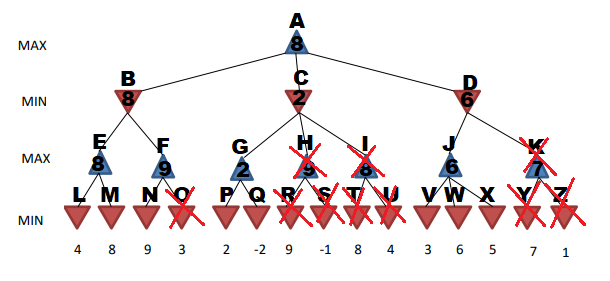
\includegraphics[width=1\linewidth]{image4.png}
\end{figure}
\end{alltt}
\end{document}
